\title{%
  DD1301 Datorintroduktion
}
\author{Daniel Bosk}
\institute{%
  KTH EECS
}

\mode<article>{\maketitle}
\mode<presentation>{%
  \begin{frame}
    \maketitle
  \end{frame}
}

\mode*


\section{What to learn?}

\subsection{Terminal}

\begin{frame}
  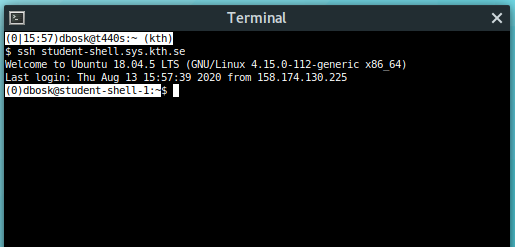
\includegraphics[width=\columnwidth]{../../terminal/terminal.png}
\end{frame}

\begin{frame}[fragile]
  \begin{lstlisting}[numbers=none]
n=10 cat hitch-hikers-guide.txt | \
  tr -cs A-Za-z '\n' | tr A-Z a-z | \
  sort | \
  uniq -c | \
  sort -rn | \
  head -n \$n
  \end{lstlisting}
\end{frame}


\subsection{Version management}

\begin{frame}
  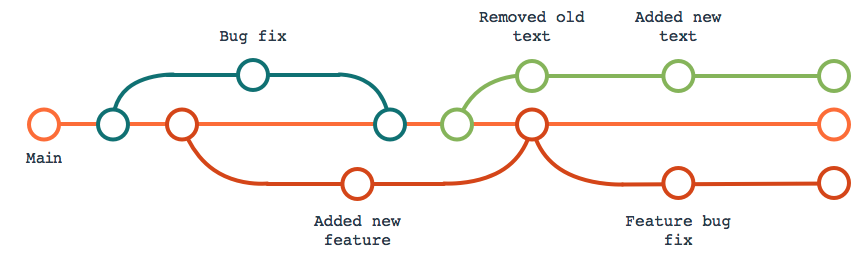
\includegraphics[width=\columnwidth]{figs/version-tree.png}
\end{frame}


\subsection{\LaTeX}

\begin{frame}
\[
  f(x, y) = \sum_{i=1}^n 
  \frac{x^{\frac{2^{2^{2^{2^n}}}}{\sqrt{1-\frac{v^2}{c^2}}}}}{y}
\]

%  \begin{lstlisting}
%R^*=\argmin_{\substack{RR^t=I,\\ \det(R)=1}}
%    \sum_{i=1}^n \omega_i \norm{RX_i-Y_i}^2_2,
%  \end{lstlisting}
\end{frame}

\begin{frame}[fragile]
  \lstinputlisting[firstline=19,firstnumber=19,lastline=37]{contents.tex}
\end{frame}


\section{The course}

\subsection{Course material}

\begin{frame}
  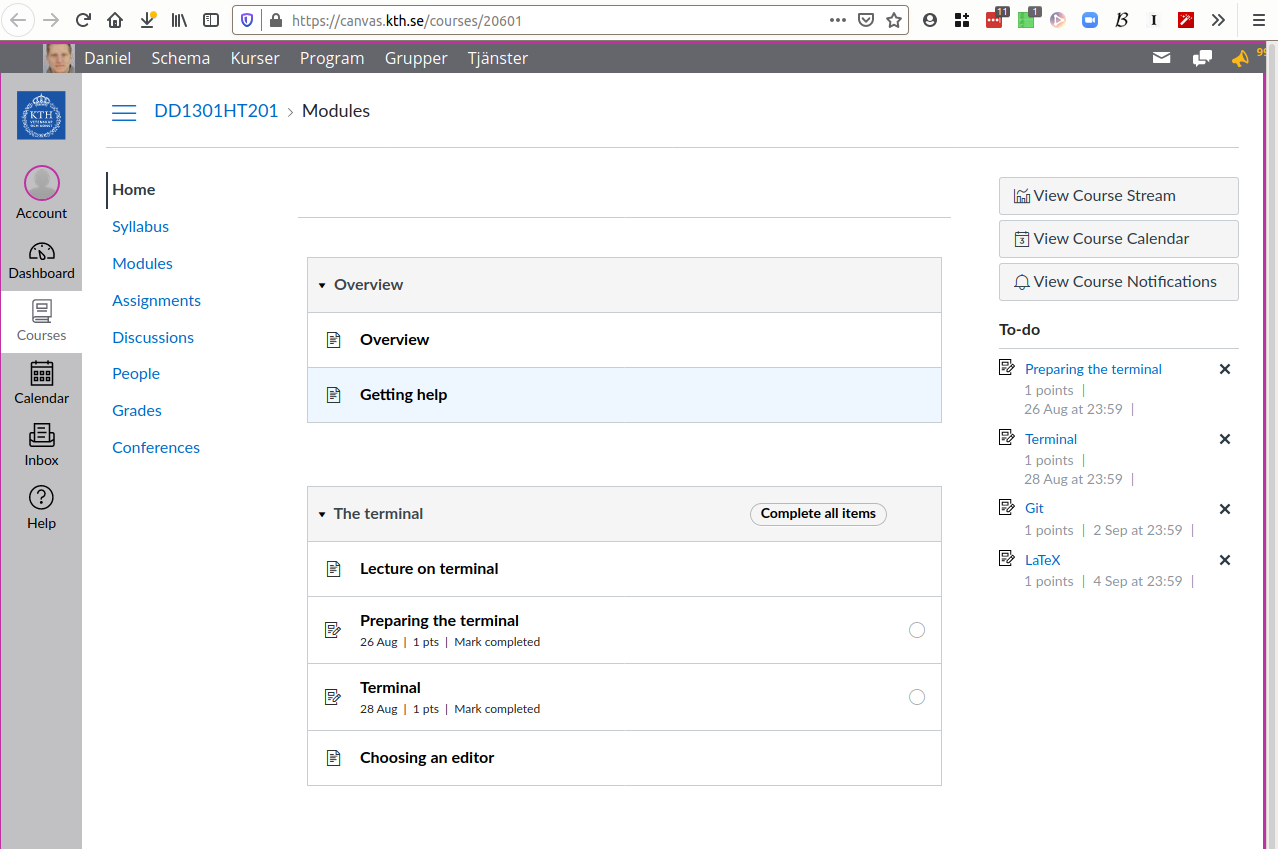
\includegraphics[width=\columnwidth]{figs/canvas.png}
\end{frame}

\subsection{The labs}

\begin{frame}
  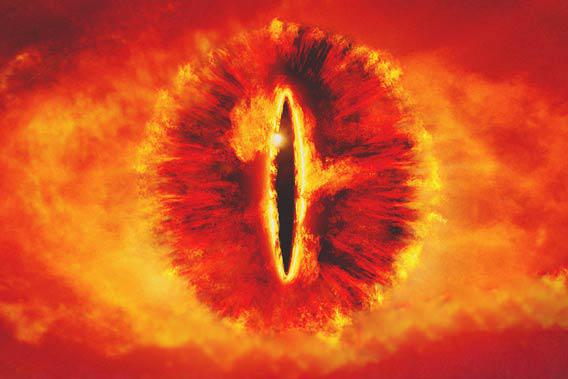
\includegraphics[width=\columnwidth]{figs/sauron.jpg}
\end{frame}


\section{Advice from previous students}

\begin{frame}
  \section{Advice from previous students}

\begin{frame}
  \begin{example}[Good for future]
    \begin{itemize}
      \item Gör uppgifterna de är nyttiga och inte särskilt svåra, bra för 
        framtida kurser
      \item Ta till dig den information som erbjuds, du kan komma att ha 
        användning för den i framtida kurser.
      \item Lär dig Git ordentligt!
      \item Om du ska använda KTH-datorer, gör kursen!
      \item Även om det var på tok för mycket överflödig info så var det som 
        man lärde sig för uppgifterna värdefullt. Till exempel så även om man 
        kanske inte använder terminalen för att pusha till github så är det bra 
        att kunna veta alternativ osv.
      \item Lägg lite mer möda på att lära sig latex eftersom man kommer vilja 
        kunna det senare ändå.
    \end{itemize}
  \end{example}
\end{frame}

\begin{frame}
  \begin{example}[When to finish?]
    \begin{itemize}
      \item Gör kursen direkt och skjut inte upp det.
      \item Gör allt på en gång och lägg ner tid på att förstå innehållet, det 
        kommer hjälpa er i framtiden väldigt mycket!
      \item Känn ingen stress att göra klart kursen under de två veckorna som 
        kursen går. Jag lade mycket tid för att få klart den på en gång vilket 
        tyvärr gjorde att jag hamnade efter i de mattekurserna som fick parallellt.
    \end{itemize}
  \end{example}
\end{frame}

\begin{frame}
  \begin{example}[Help?]
    \begin{itemize}
      \item Försök att göra klart uppgifterna under tiden det finns 
        handledning.
      \item Utnyttja den hjälp som finns, de kan ofta lösa diverse tekniska 
        problem.
      \item Googla errormeddelandena och fråga också på canvas, var tydlig med 
        vad du har gjort och vad datorn klagar på. Ta screenshots.
    \end{itemize}
  \end{example}
\end{frame}


\end{frame}

%%% REFERENCES %%%

\begin{frame}[allowframebreaks]
  \printbibliography{}
\end{frame}
